\documentclass{article}
% Adjust the relative path to point to the latex-templates directory

% content/resources/templates/preamble.tex
\usepackage[margin=0.6in]{geometry}
\author{Milav Dabgar}
\usepackage{amsmath,amssymb,amsthm}
\usepackage{booktabs}
\usepackage{multirow}
\usepackage{xcolor}
\usepackage{tcolorbox}
\tcbuselibrary{breakable,skins}
\usepackage[colorlinks=true,linkcolor=blue]{hyperref}
\usepackage{titlesec}
\usepackage{enumitem}
\usepackage{tikz}
\usepackage{pgfplots}
\usepackage{circuitikz}
\usepackage[version=4]{mhchem}
\usepackage{longtable}
\usepackage{array}
\usepackage{float}
\usepackage{caption}
\usepackage{listings}

\lstset{
  basicstyle=\small\ttfamily,
  breaklines=true,
  breakatwhitespace=false,
  postbreak=\mbox{\textcolor{red}{$\hookrightarrow$}\space},
  float=false,
  numbers=left,
  numberstyle=\tiny\color{gray},
  numbersep=10pt,
  xleftmargin=2em,
  keywordstyle=\color{blue},
  commentstyle=\color{green!60!black},
  stringstyle=\color{purple},
  backgroundcolor=\color{gray!5},
  showstringspaces=false,
  tabsize=2,
  captionpos=b,
  keepspaces=true,
  columns=flexible
}

\pgfplotsset{compat=1.18}
\usetikzlibrary{shapes,arrows,positioning,calc,patterns,decorations.pathmorphing,decorations.markings,arrows.meta}

% Color scheme
\definecolor{headcolor}{RGB}{0,102,204}
\definecolor{keycolor}{RGB}{220,20,60}
\definecolor{solutioncolor}{RGB}{34,139,34}
\definecolor{mnemoniccolor}{RGB}{148,0,211}
\definecolor{codecolor}{RGB}{0,0,100}

% Spacing
\setlength{\parskip}{3pt}
\setlist[itemize]{nosep}
\setlist[enumerate]{nosep}

% Title formatting
\titleformat{\section}{\Large\bfseries\color{headcolor}}{\thesection}{1em}{}
\titleformat{\subsection}{\large\bfseries\color{headcolor}}{\thesubsection}{1em}{}

% Pandoc tightlist compatibility
\providecommand{\tightlist}{%
  \setlength{\itemsep}{0pt}\setlength{\parskip}{0pt}}

% Pandoc longtable compatibility
\newcounter{none}
\def\thenone{}


% content/resources/templates/english-boxes.tex

% Custom environments
\newtcolorbox{solutionbox}{
 breakable,
 enhanced,
 colback=solutioncolor!5!white,
 colframe=solutioncolor!75!black,
 fonttitle=\bfseries,
 title=Solution
}

\newtcolorbox{solutionboxnobreak}{
 colback=solutioncolor!5!white,
 colframe=solutioncolor!75!black,
 fonttitle=\bfseries,
 title=Solution
}

\newtcolorbox{keyformula}{
 breakable,
 enhanced,
 colback=keycolor!5!white,
 colframe=keycolor!75!black,
 fonttitle=\bfseries,
 title=Key Formula
}

\newtcolorbox{mnemonicboxenv}{
 breakable,
 enhanced,
 colback=mnemoniccolor!5!white,
 colframe=mnemoniccolor!75!black,
 fonttitle=\bfseries,
 title=Mnemonic
}

\newcommand{\mnemonicbox}[1]{%
  \begin{mnemonicboxenv}
    #1
  \end{mnemonicboxenv}
}


% Custom commands for GTU solutions
% This file defines semantic commands for consistent formatting

% Question command with automatic formatting
\newcommand{\question}[2]{%
  \section*{Question #1}%
  \textbf{#2}%
}

% OR question variant
\newcommand{\questionor}[2]{%
  \section*{Question #1 OR}%
  \textbf{#2}%
}

% Proper table environment with caption
\newenvironment{answertable}[1]{%
  \begin{table}[htbp]
  \centering
  \caption{#1}
}{%
  \end{table}
}

% Proper figure environment for diagrams
\newenvironment{answerdiagram}[1]{%
  \begin{figure}[htbp]
  \centering
  \caption{#1}
}{%
  \end{figure}
}

% Semantic markup for key terms
\newcommand{\keyword}[1]{\textbf{#1}}
\newcommand{\code}[1]{\texttt{#1}}
\newcommand{\classname}[1]{\texttt{#1}}
\newcommand{\methodname}[1]{\texttt{#1}}

% Proper quotation marks
\newcommand{\mnemonic}[1]{``#1''}


\title{Fundamentals of Electronics (4311102) - Winter 2023 Solution}
\date{January 24, 2023}

\begin{document}
\maketitle

\questionmarks{1(a)}{3}{Define Forward and reverse bias of diode.}

\begin{solutionbox}
\textbf{Answer}:

\textbf{Forward Bias of Diode}: 

\begin{itemize}
    \item \keyword{Connection Method}: P-type connected to positive terminal and N-type connected to negative terminal of battery
    \item \keyword{Barrier Width}: Barrier width decreases
    \item \keyword{Resistance}: Low resistance (typically 100-1000$\Omega$)
    \item \keyword{Current Flow}: Allows current to flow easily through the diode
\end{itemize}

\textbf{Reverse Bias of Diode}:

\begin{itemize}
    \item \keyword{Connection Method}: P-type connected to negative terminal and N-type connected to positive terminal
    \item \keyword{Barrier Width}: Barrier width increases
    \item \keyword{Resistance}: Very high resistance (typically several M$\Omega$)
    \item \keyword{Current Flow}: Blocks current flow (only small leakage current flows)
\end{itemize}

\textbf{Diagram}:

\begin{center}
\begin{tikzpicture}[node distance=2.5cm, auto]
    \node [gtu state] (Fwd) {Forward Bias};
    \node [gtu block, right=1cm of Fwd, text width=4cm] (FwdDesc) {P connected to +ve\\N connected to -ve};
    \node [gtu block, right=1cm of FwdDesc] (FwdRes) {Current flows easily};
    
    \node [gtu state, below=1.5cm of Fwd] (Rev) {Reverse Bias};
    \node [gtu block, right=1cm of Rev, text width=4cm] (RevDesc) {P connected to -ve\\N connected to +ve};
    \node [gtu block, right=1cm of RevDesc] (RevRes) {Current blocked};

    \path [gtu arrow] (Fwd) -- (FwdDesc);
    \path [gtu arrow] (FwdDesc) -- (FwdRes);
    \path [gtu arrow] (Rev) -- (RevDesc);
    \path [gtu arrow] (RevDesc) -- (RevRes);
\end{tikzpicture}
\captionof{figure}{Forward and Reverse Bias Logic}
\end{center}
\end{solutionbox}

\begin{mnemonicbox}
\mnemonic{PFNR: "Positive to P Forward, Negative to P Reverse"}
\end{mnemonicbox}

\questionmarks{1(b)}{4}{Explain construction and working of LDR.}

\begin{solutionbox}
\textbf{Answer}:

\textbf{Construction of LDR}:

\begin{itemize}
    \item \keyword{Material}: Made of semiconductor material (Cadmium Sulfide)
    \item \keyword{Pattern}: Zigzag pattern of photosensitive material on ceramic base
    \item \keyword{Electrodes}: Metal electrodes at both ends
    \item \keyword{Package}: Encapsulated in transparent plastic or glass case
\end{itemize}

\textbf{Working Principle}:

\begin{itemize}
    \item \keyword{Photoconductivity}: Based on photoconductivity principle
    \item \keyword{Dark Resistance}: High resistance (M$\Omega$ range) in dark conditions
    \item \keyword{Light Exposure}: When exposed to light, photons release electrons 
    \item \keyword{Resistance Drop}: Resistance decreases (k$\Omega$ range) in bright light
\end{itemize}

\textbf{Diagram}:

\begin{center}
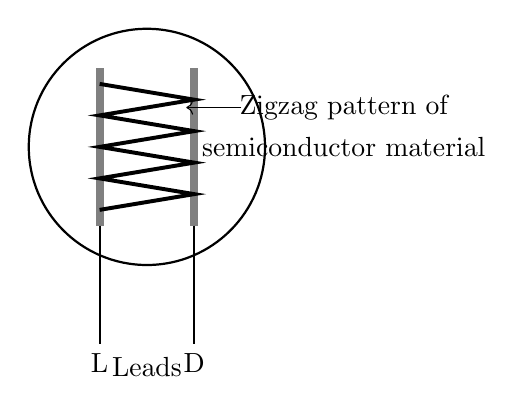
\begin{tikzpicture}
    % Ceramic Base
    \draw[fill=white, thick] (0,0) circle (1.5cm);
    
    % Electrodes (Zigzag)
    \draw[line width=1mm, color=gray] (-0.6, 1) -- (-0.6, -1);
    \draw[line width=1mm, color=gray] (0.6, 1) -- (0.6, -1);
    
    % Zigzag track
    \draw[line width=0.5mm] (-0.6, 0.8) -- (0.6, 0.6) -- (-0.6, 0.4) -- (0.6, 0.2) -- (-0.6, 0) -- (0.6, -0.2) -- (-0.6, -0.4) -- (0.6, -0.6) -- (-0.6, -0.8);
    
    \node at (2.5, 0.5) {Zigzag pattern of};
    \node at (2.5, 0) {semiconductor material};
    \draw[->] (1.2, 0.5) -- (0.5, 0.5);

    % Leads
    \draw[thick] (-0.6, -1) -- (-0.6, -2.5) node[below] {L};
    \draw[thick] (0.6, -1) -- (0.6, -2.5) node[below] {D};
    \node at (0, -2.8) {Leads};
\end{tikzpicture}
\captionof{figure}{LDR Construction}
\end{center}
\end{solutionbox}

\begin{mnemonicbox}
\mnemonic{MILD: "More Illumination, Less Dark-resistance"}
\end{mnemonicbox}

\questionmarks{1(c)}{7}{Explain the color band coding method of Resistor. Write color band of 47k$\Omega$ $\pm$5\% resistance.}

\begin{solutionbox}
\textbf{Answer}:

\textbf{Color Band Coding Method}:

\begin{center}
\captionof{table}{Resistor Color Code}
\begin{tabulary}{\linewidth}{|L|L|L|L|}
\hline
\textbf{Color} & \textbf{Value} & \textbf{Multiplier} & \textbf{Tolerance} \\ \hline
Black & 0 & $10^0$ & - \\ \hline
Brown & 1 & $10^1$ & $\pm1\%$ \\ \hline
Red & 2 & $10^2$ & $\pm2\%$ \\ \hline
Orange & 3 & $10^3$ & - \\ \hline
Yellow & 4 & $10^4$ & - \\ \hline
Green & 5 & $10^5$ & $\pm0.5\%$ \\ \hline
Blue & 6 & $10^6$ & $\pm0.25\%$ \\ \hline
Violet & 7 & $10^7$ & $\pm0.1\%$ \\ \hline
Grey & 8 & $10^8$ & $\pm0.05\%$ \\ \hline
White & 9 & $10^9$ & - \\ \hline
Gold & - & $10^{-1}$ & $\pm5\%$ \\ \hline
Silver & - & $10^{-2}$ & $\pm10\%$ \\ \hline
Colorless & - & - & $\pm20\%$ \\ \hline
\end{tabulary}
\end{center}

\textbf{4-Band Resistor Color Code}:

\begin{itemize}
    \item \keyword{First Band}: First significant digit
    \item \keyword{Second Band}: Second significant digit
    \item \keyword{Third Band}: Multiplier
    \item \keyword{Fourth Band}: Tolerance
\end{itemize}

\textbf{For 47k$\Omega$ $\pm$5\%}:

\begin{itemize}
    \item First digit: 4 = Yellow
    \item Second digit: 7 = Violet
    \item Multiplier: $10^3$ = Orange (for k$\Omega$)
    \item Tolerance: $\pm5\%$ = Gold
\end{itemize}

\textbf{Color bands for 47k$\Omega$ $\pm$5\%}: Yellow-Violet-Orange-Gold

\textbf{Diagram}:

\begin{center}
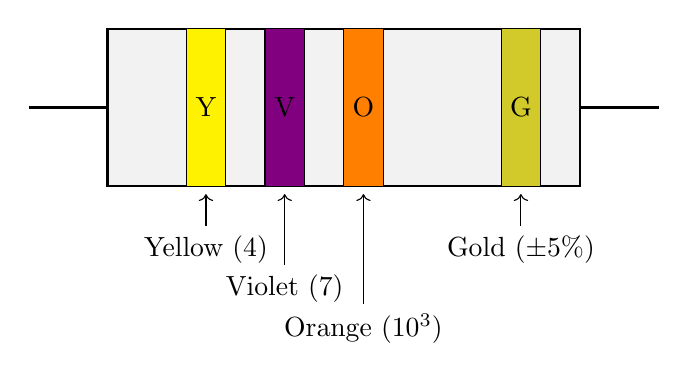
\begin{tikzpicture}
    % Resistor Body
    \draw[thick, fill=gray!10] (0,0) rectangle (6,2);
    \draw[thick] (-1, 1) -- (0, 1);
    \draw[thick] (6, 1) -- (7, 1);
    
    % Bands
    \foreach \x/\c/\t in {1/yellow/Y, 2/violet/V, 3/orange/O, 5/yellow!80!black/G} {
        \draw[fill=\c] (\x,0) rectangle (\x+0.5,2);
        \node at (\x+0.25, 1) {\t};
    }
    
    % Callouts
    \draw[<-] (1.25, -0.1) -- (1.25, -0.5) node[below] {Yellow (4)};
    \draw[<-] (2.25, -0.1) -- (2.25, -1) node[below] {Violet (7)};
    \draw[<-] (3.25, -0.1) -- (3.25, -1.5) node[below] {Orange ($10^3$)};
    \draw[<-] (5.25, -0.1) -- (5.25, -0.5) node[below] {Gold ($\pm5\%$)};
\end{tikzpicture}
\captionof{figure}{Resistor Color Bands: Yellow-Violet-Orange-Gold}
\end{center}
\end{solutionbox}

\begin{mnemonicbox}
\mnemonic{BAND: "Beginning digits, Amplify with Multiplier, Note tolerance with last band, Decode carefully"}
\end{mnemonicbox}

\questionmarks{1(c OR)}{7}{Explain Aluminum Electrolytic wet type capacitor.}

\begin{solutionbox}
\textbf{Answer}:

\textbf{Aluminum Electrolytic Wet Type Capacitor}:

\textbf{Construction}:

\begin{itemize}
    \item \keyword{Plates}: Two aluminum foils (anode and cathode)
    \item \keyword{Dielectric}: Aluminum oxide layer on anode foil
    \item \keyword{Electrolyte}: Liquid electrolyte (boric acid, sodium borate, etc.)
    \item \keyword{Separator}: Paper separator soaked in electrolyte
    \item \keyword{Enclosure}: Aluminum can with rubber seal
\end{itemize}

\textbf{Working Principle}:

\begin{itemize}
    \item \keyword{Oxide Layer}: Thin aluminum oxide layer acts as dielectric
    \item \keyword{Electrolyte}: Acts as cathode connection to second plate
    \item \keyword{Polarization}: Has defined polarity (+ and -) terminals
\end{itemize}

\textbf{Characteristics}:

\begin{itemize}
    \item \keyword{Capacitance Range}: 1$\mu$F to 47,000$\mu$F
    \item \keyword{Voltage Rating}: 6.3V to 450V
    \item \keyword{Polarity}: Polarized (must connect correctly)
    \item \keyword{Leakage Current}: Higher than other capacitor types
    \item \keyword{ESR}: Higher equivalent series resistance
\end{itemize}

\textbf{Diagram}:

\begin{center}
\begin{tikzpicture}[node distance=1.5cm]
    \node [gtu state, align=center] (Cap) {Aluminum Electrolytic\\Capacitor};
    
    \node [gtu block, below left=1cm of Cap] (Anode) {Anode Foil\\(Aluminum)};
    \node [gtu block, below right=1cm of Cap] (Cathode) {Cathode Foil\\(Aluminum)};
    \node [gtu block, below=2cm of Cap] (Elec) {Electrolyte\\(Liquid)};
    \node [gtu block, left=1cm of Anode] (Oxide) {Oxide Layer\\(Dielectric)};
    \node [gtu block, right=1cm of Cathode] (Sep) {Separator\\(Paper)};

    \path [gtu arrow] (Cap) -- (Anode);
    \path [gtu arrow] (Cap) -- (Cathode);
    \path [gtu arrow] (Cap) -- (Elec);
    \path [gtu arrow] (Anode) -- (Oxide);
    \path [gtu arrow] (Cap) -- (Sep);
\end{tikzpicture}
\captionof{figure}{Aluminum Electrolytic Capacitor Components}
\end{center}
\end{solutionbox}

\begin{mnemonicbox}
\mnemonic{POLE: "Polarized, Oxide layer, Liquid electrolyte, Enormous capacitance"}
\end{mnemonicbox}

\questionmarks{2(a)}{3}{Draw the symbol of Schottkey diode, LED and Photo-diode.}

\begin{solutionbox}
\textbf{Answer}:

\textbf{Symbols}:

\begin{center}
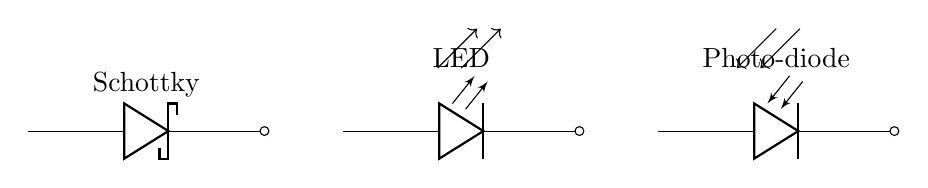
\begin{tikzpicture}
    % Schottky
    \draw (0,0) to[Schottky diode, l=Schottky, -o] (3,0);
    
    % LED
    \draw (4,0) to[led, l=LED, -o] (7,0);
    \draw[->] (5.5, 0.8) -- (6, 1.3);
    \draw[->] (5.2, 0.8) -- (5.7, 1.3);
    
    % Photo-diode
    \draw (8,0) to[photodiode, l=Photo-diode, -o] (11,0);
    \draw[->] (9.5, 1.3) -- (9, 0.8);
    \draw[->] (9.8, 1.3) -- (9.3, 0.8);
\end{tikzpicture}
\captionof{figure}{Symbols: Schottky Diode, LED, Photo-diode}
\end{center}

\textbf{Key Features}:

\begin{itemize}
    \item \keyword{Schottky Diode}: Standard diode symbol with curved bar (represents metal-semiconductor junction)
    \item \keyword{LED}: Standard diode symbol with two arrows pointing away (represents light emission)
    \item \keyword{Photo-diode}: Standard diode symbol with two arrows pointing toward diode (represents light detection)
\end{itemize}
\end{solutionbox}

\begin{mnemonicbox}
\mnemonic{SLP: "Schottky has curve, LED emits, Photo-diode absorbs"}
\end{mnemonicbox}

\questionmarks{2(b)}{4}{Define Active and Passive Components with example.}

\begin{solutionbox}
\textbf{Answer}:

\textbf{Passive Components}:

\begin{center}
\captionof{table}{Passive vs Active Components}
\begin{tabulary}{\linewidth}{|L|L|L|}
\hline
\textbf{Characteristic} & \textbf{Description} & \textbf{Examples} \\ \hline
\multicolumn{3}{|c|}{\textbf{Passive Components}} \\ \hline
Power & Cannot generate power & Resistors, Capacitors, Inductors \\ \hline
Signal & Cannot amplify signals & Transformers, Diodes \\ \hline
Control & No control over current flow & Connectors, Switches \\ \hline
Energy & Store or dissipate energy & Fuses, Filters \\ \hline
\multicolumn{3}{|c|}{\textbf{Active Components}} \\ \hline
Power & Can generate power & Transistors, ICs \\ \hline
Signal & Can amplify signals & Op-amps, Amplifiers \\ \hline
Control & Control current flow & SCRs, MOSFETs \\ \hline
Dependency & Require external power & Voltage regulators, Microcontrollers \\ \hline
\end{tabulary}
\end{center}

\textbf{Diagram}:

\begin{center}
\begin{tikzpicture}[node distance=1.5cm]
    \node [gtu block] (Main) {Electronic Components};
    \node [gtu block, below left=1.0cm of Main] (Active) {Active Components\\(Control/Amplify)};
    \node [gtu block, below right=1.0cm of Main] (Passive) {Passive Components\\(Store/Dissipate)};
    
    \node [gtu state, below=0.5cm of Active] (ActEx) {Transistor, IC, SCR};
    \node [gtu state, below=0.5cm of Passive] (PasEx) {Resistor, Capacitor, Inductor};
    
    \path [gtu arrow] (Main) -- (Active);
    \path [gtu arrow] (Main) -- (Passive);
    \path [gtu arrow] (Active) -- (ActEx);
    \path [gtu arrow] (Passive) -- (PasEx);
\end{tikzpicture}
\captionof{figure}{Classification of Electronic Components}
\end{center}
\end{solutionbox}

\begin{mnemonicbox}
\mnemonic{PASS-ACT: "Passive stores or dissipates, Active controls or amplifies"}
\end{mnemonicbox}

\questionmarks{2(c)}{7}{Explain working of full wave bridge rectifier.}

\begin{solutionbox}
\textbf{Answer}:

\textbf{Full Wave Bridge Rectifier}:

\textbf{Circuit Construction}:

\begin{itemize}
    \item \keyword{Diodes}: Four diodes arranged in bridge configuration
    \item \keyword{Input}: AC supply from transformer secondary
    \item \keyword{Output}: Pulsating DC across load resistor with filter capacitor
\end{itemize}

\textbf{Working Principle}:

\begin{itemize}
    \item \keyword{Positive Half Cycle}: D1 and D3 conduct, D2 and D4 block
    \item \keyword{Negative Half Cycle}: D2 and D4 conduct, D1 and D3 block
    \item \keyword{Current Flow}: Always flows through load in same direction
\end{itemize}

\textbf{Performance Parameters}:

\begin{itemize}
    \item \keyword{Ripple Frequency}: 2$\times$ input frequency (100 Hz for 50 Hz input)
    \item \keyword{Efficiency}: 81.2\%
    \item \keyword{PIV}: $V_0(max)$ per diode
    \item \keyword{TUF}: 0.812 (Transformer Utilization Factor)
\end{itemize}

\textbf{Diagram}:

\begin{center}
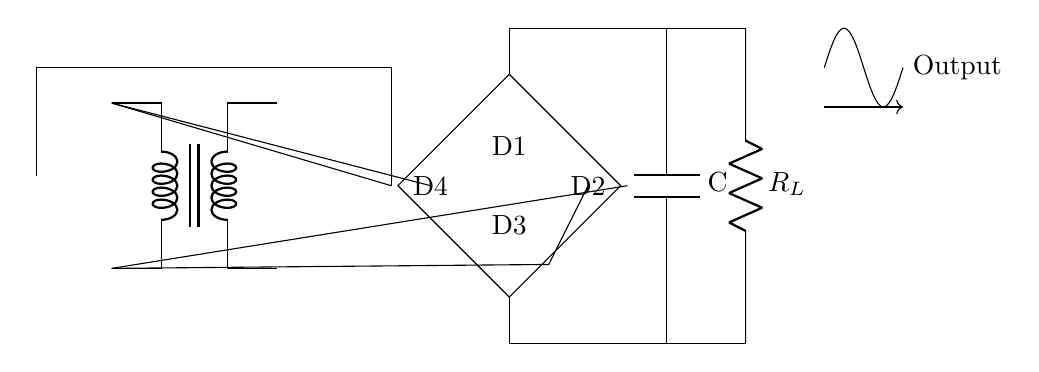
\begin{tikzpicture}
    % Circuit
    % Transformer
    \draw (0,0) node[transformer core] (T) {};
    
    % Bridge Nodes
    \coordinate (Top) at (4, 1.5);
    \coordinate (Right) at (5.5, 0);
    \coordinate (Bottom) at (4, -1.5);
    \coordinate (Left) at (2.5, 0);
    
    % Connections from Transformer
    \draw (T.A1) -- (Left);
    \draw (T.A2) -- (Right); % Wait, this shorts the bridge. Correct: AC to opposite corners.
    % In bridge: AC applied to Input terminals (Left/Right), DC taken from Top/Bottom? Or vice versa.
    % Standard: 4 diodes D1,D2,D3,D4.
    % Let's draw standard diamond properly.
    
    % Let's restart bridge drawing for clarity
    % AC Source
    \draw (-2, 0) node[sV, l=AC Input] (AC) {};
    \draw (AC.north) -- (-2, 1.5) -- (2.5, 1.5) -- (2.5, 0); % To Left Node of Bridge?
    % No, allow me to simplify: Transformer -> Bridge Block -> Load
    
    \node[draw, minimum width=2cm, minimum height=2cm, rotate=45] (Bridge) at (4,0) {};
    \node at (4,0.5) {D1}; \node at (5,0) {D2};
    \node at (4,-0.5) {D3}; \node at (3,0) {D4};
    
    % Connecitons
    \draw (T.A1) -- (3,0); % Left point of diamond (AC In 1)
    \draw (T.A2) to[jump crossing] (4.5,-1) -- (5,0); % Right point of diamond (AC In 2) - visual approx
    
    % DC Out
    \draw (4, 1.414) -- (4, 2) -- (7, 2); % Top point (DC+)
    \draw (4, -1.414) -- (4, -2) -- (7, -2); % Bottom point (DC-)
    
    % Load
    \draw (7, 2) to[R, l=$R_L$] (7, -2);
    
    % Filter Cap
    \draw (6, 2) to[C, l=C] (6, -2);
    
    % Waveforms
    \draw[->] (8, 1) -- (9, 1);
    \draw (8, 1.5) sin (8.25, 2) cos (8.5, 1.5) sin (8.75, 1) cos (9, 1.5); % Output (DC)
    \node[right] at (9,1.5) {Output};

\end{tikzpicture}
\captionof{figure}{Full Wave Bridge Rectifier Circuit}
\end{center}
\end{solutionbox}

\begin{mnemonicbox}
\mnemonic{BRIDGE: "Better Rectification with Improved Diode Geometry Efficiency"}
\end{mnemonicbox}

\questionmarks{2(a OR)}{3}{Explain construction and working of LED.}

\begin{solutionbox}
\textbf{Answer}:

\textbf{Construction of LED}:

\begin{itemize}
    \item \keyword{Material}: Semiconductor (GaAs, GaP, AlGaInP, etc.)
    \item \keyword{Junction}: P-N junction with heavily doped semiconductors
    \item \keyword{Package}: Encased in transparent or colored epoxy lens
    \item \keyword{Cathode}: Identified by flat side on package or shorter lead
\end{itemize}

\textbf{Working Principle}:

\begin{itemize}
    \item \keyword{Forward Bias}: Applied to P-N junction
    \item \keyword{Recombination}: Electrons and holes recombine at junction
    \item \keyword{Energy Release}: Energy released as photons (light)
    \item \keyword{Wavelength}: Determined by band gap of semiconductor material
\end{itemize}

\textbf{Diagram}:

\begin{center}
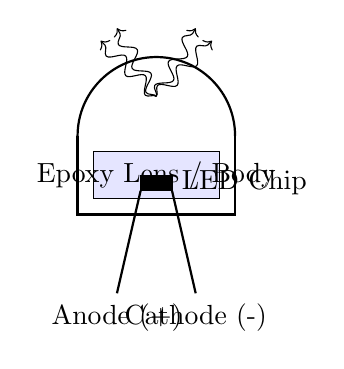
\begin{tikzpicture}
    % Construction
    \draw[thick] (0,0) arc (180:0:1);
    \draw[thick] (0,0) -- (0,-1) -- (2,-1) -- (2,0);
    
    \draw[fill=blue!10] (0.2, -0.2) rectangle (1.8, -0.8);
    \node at (1, -0.5) {Epoxy Lens / Body};
    
    \draw[fill=black] (0.8, -0.5) rectangle (1.2, -0.7);
    \node[right] at (1.2, -0.6) {LED Chip};
    
    \draw[thick] (0.8, -0.7) -- (0.5, -2) node[below] {Anode (+)};
    \draw[thick] (1.2, -0.7) -- (1.5, -2) node[below] {Cathode (-)};
    
    % Light
    \foreach \angle in {45, 60, 120, 135}
        \draw[->, decorate, decoration={snake}] (1, 0.5) -- ++(\angle:1);
\end{tikzpicture}
\captionof{figure}{LED Construction}
\end{center}
\end{solutionbox}

\begin{mnemonicbox}
\mnemonic{LEDS: "Light Emits During electron-hole recombination in Semiconductor"}
\end{mnemonicbox}

\questionmarks{2(b OR)}{4}{Explain composition type resistors.}

\begin{solutionbox}
\textbf{Answer}:

\textbf{Composition Resistors}:

\textbf{Construction}:

\begin{itemize}
    \item \keyword{Core Material}: Carbon particles mixed with insulating material (clay/ceramic)
    \item \keyword{Binding}: Resin binder forms solid cylindrical shape
    \item \keyword{Terminals}: Metal caps with leads attached to ends
    \item \keyword{Protection}: Coated with insulating paint or plastic
\end{itemize}

\textbf{Characteristics}:

\begin{itemize}
    \item \keyword{Resistance Range}: 1$\Omega$ to 22M$\Omega$
    \item \keyword{Power Rating}: 1/8W to 2W
    \item \keyword{Tolerance}: $\pm$5\% to $\pm$20\%
    \item \keyword{Temperature Coefficient}: -500 to +500 ppm/$^{\circ}$C
\end{itemize}

\textbf{Advantages \& Limitations}:

\begin{itemize}
    \item \keyword{Cost}: Low cost
    \item \keyword{Noise}: Higher noise level
    \item \keyword{Stability}: Less stable with temperature
    \item \keyword{Applications}: General purpose, non-critical applications
\end{itemize}

\textbf{Diagram}:

\begin{center}
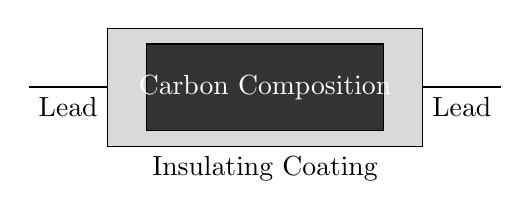
\begin{tikzpicture}
    \draw[fill=gray!30] (0,0) rectangle (4,1.5);
    \draw[fill=black!80] (0.5, 0.2) rectangle (3.5, 1.3);
    \node[white] at (2, 0.75) {Carbon Composition};
    \node[below] at (2, 0) {Insulating Coating};
    
    \draw[thick] (-1, 0.75) -- (0, 0.75);
    \draw[thick] (4, 0.75) -- (5, 0.75);
    \node[below] at (-0.5, 0.75) {Lead};
    \node[below] at (4.5, 0.75) {Lead};
\end{tikzpicture}
\captionof{figure}{Carbon Composition Resistor Structure}
\end{center}
\end{solutionbox}

\begin{mnemonicbox}
\mnemonic{CCRI: "Carbon Composition Resistors are Inexpensive"}
\end{mnemonicbox}

\questionmarks{2(c OR)}{7}{Explain working of full wave rectifier with two diodes.}

\begin{solutionbox}
\textbf{Answer}:

\textbf{Full Wave Rectifier with Two Diodes (Center-tap)}:

\textbf{Circuit Construction}:

\begin{itemize}
    \item \keyword{Transformer}: Center-tapped transformer secondary
    \item \keyword{Diodes}: Two diodes connected to opposite ends of secondary
    \item \keyword{Output}: Taken between center tap and diode junction
\end{itemize}

\textbf{Working Principle}:

\begin{itemize}
    \item \keyword{Positive Half Cycle}: Upper half of secondary positive, D1 conducts, D2 blocks
    \item \keyword{Negative Half Cycle}: Lower half of secondary positive, D2 conducts, D1 blocks
    \item \keyword{Current Flow}: Always flows through load in same direction
\end{itemize}

\textbf{Performance Parameters}:

\begin{itemize}
    \item \keyword{Ripple Frequency}: 2$\times$ input frequency (100 Hz for 50 Hz input)
    \item \keyword{Efficiency}: 81.2\%
    \item \keyword{PIV}: $2V_0(max)$ per diode (twice the center-tap rectifier)
    \item \keyword{TUF}: 0.693 (Transformer Utilization Factor)
\end{itemize}

\textbf{Diagram}:

\begin{center}
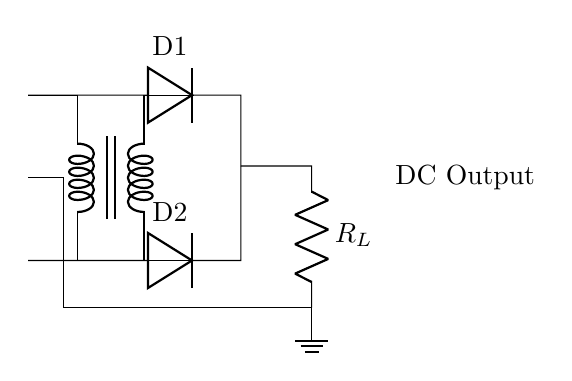
\begin{tikzpicture}[scale=0.9]
    \draw (0,0) node[transformer core] (T) {};
    
    % Secondary Top
    \draw (T.A1) -- ++(1,0) to[diode, l=D1] ++(2,0) -- ++(0,-1) coordinate (Junc);
    
    % Secondary Bottom
    \draw (T.A2) -- ++(1,0) to[diode, l=D2] ++(2,0) -- ++(0,1) -- (Junc);
    
    % Load
    \draw (Junc) -- ++(1,0) to[R, l=$R_L$] ++(0,-2) coordinate (GND_Node);
    
    % Center Tap
    % Circuitikz transformer anchors: A1 top sec, A2 bottom sec. Center tap needs creating visual or finding anchor?
    % Visual approximation
    \coordinate (CT) at ($(T.A1)!0.5!(T.A2)$);
    \draw (CT) -- ++(0.5,0) |- (GND_Node);
    \node[ground] at (GND_Node) {};
    
    % Labels
    \node at (5, 0) {DC Output};
\end{tikzpicture}
\captionof{figure}{Center-Tap Full Wave Rectifier}
\end{center}
\end{solutionbox}

\begin{mnemonicbox}
\mnemonic{CTFWR: "Center Tap Facilitates Whole-cycle Rectification"}
\end{mnemonicbox}

\questionmarks{3(a)}{3}{Explain working of schhotkey diode.}

\begin{solutionbox}
\textbf{Answer}:

\textbf{Working of Schottky Diode}:

\begin{itemize}
    \item \keyword{Junction Type}: Metal-Semiconductor (M-S) junction instead of P-N
    \item \keyword{Charge Carriers}: Majority carrier device (electrons in N-type)
    \item \keyword{Barrier}: Schottky barrier formed at metal-semiconductor interface
    \item \keyword{Forward Voltage}: Lower forward voltage drop (0.2-0.4V vs 0.7V for Si diode)
\end{itemize}

\textbf{Key Characteristics}:

\begin{itemize}
    \item \keyword{Switching Speed}: Very fast switching (no minority carrier storage)
    \item \keyword{Applications}: High-frequency circuits, power supplies
    \item \keyword{Recovery Time}: Negligible reverse recovery time
\end{itemize}

\textbf{Diagram}:

\begin{center}
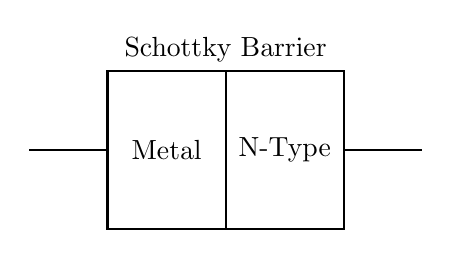
\begin{tikzpicture}
    \draw[thick] (0,0) rectangle (1.5,2);
    \node at (0.75, 1) {Metal};
    \draw[thick] (1.5,0) rectangle (3,2);
    \node at (2.25, 1) {N-Type};
    
    \draw[dashed] (1.5, 0) -- (1.5, 2);
    \node[above] at (1.5, 2) {Schottky Barrier};
    
    \draw[thick] (0, 1) -- (-1, 1);
    \draw[thick] (3, 1) -- (4, 1);
\end{tikzpicture}
\captionof{figure}{Schottky Structure}
\end{center}
\end{solutionbox}

\begin{mnemonicbox}
\mnemonic{SFAM: "Schottky's Fast And Metal-based"}
\end{mnemonicbox}

\questionmarks{3(b)}{4}{Explain N type semiconductor.}

\begin{solutionbox}
\textbf{Answer}:

\textbf{N-type Semiconductor}:

\textbf{Formation}:

\begin{itemize}
    \item \keyword{Base Material}: Intrinsic semiconductor (Silicon or Germanium)
    \item \keyword{Doping Element}: Pentavalent impurity (P, As, Sb)
    \item \keyword{Doping Process}: Thermal diffusion or ion implantation
    \item \keyword{Concentration}: Typically 1 part impurity to $10^8$ parts silicon
\end{itemize}

\textbf{Characteristics}:

\begin{itemize}
    \item \keyword{Majority Carriers}: Electrons (negative charge carriers)
    \item \keyword{Minority Carriers}: Holes
    \item \keyword{Conductivity}: Higher than intrinsic semiconductor
    \item \keyword{Fermi Level}: Closer to conduction band
\end{itemize}

\textbf{Diagram}:

\begin{center}
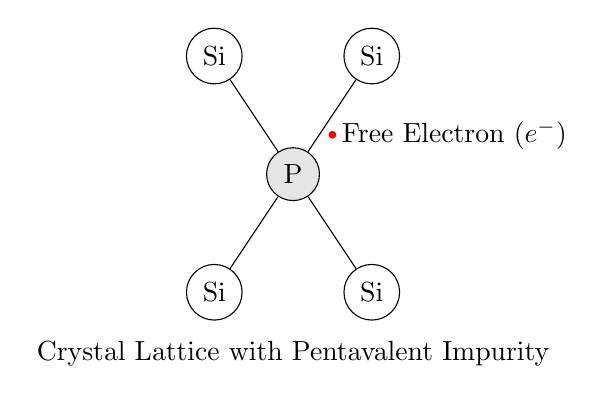
\begin{tikzpicture}
    \node[draw, circle] (Si1) at (0,0) {Si};
    \node[draw, circle] (Si2) at (2,0) {Si};
    \node[draw, circle, fill=gray!20] (P) at (1,1.5) {P};
    \node[draw, circle] (Si3) at (0,3) {Si};
    \node[draw, circle] (Si4) at (2,3) {Si};
    
    \draw (Si1) -- (P); \draw (Si2) -- (P); \draw (Si3) -- (P); \draw (Si4) -- (P);
    
    \node[circle, fill=red, inner sep=1pt] (e) at (1.5, 2) {};
    \node[right] at (e) {Free Electron ($e^-$)};
    
    \node[below] at (1, -0.5) {Crystal Lattice with Pentavalent Impurity};
\end{tikzpicture}
\captionof{figure}{N-Type Doping}
\end{center}
\end{solutionbox}

\begin{mnemonicbox}
\mnemonic{PENT: "Pentavalent Element makes N-Type with free electrons"}
\end{mnemonicbox}

\questionmarks{3(c)}{7}{Explain construction and working of PN Junction Diode.}

\begin{solutionbox}
\textbf{Answer}:

\textbf{Construction of PN Junction Diode}:

\begin{itemize}
    \item \keyword{Materials}: P-type and N-type semiconductor regions
    \item \keyword{Junction}: Formed by diffusion or epitaxial growth
    \item \keyword{Depletion Region}: Forms at junction interface
    \item \keyword{Contacts}: Metal contacts attached to both regions
    \item \keyword{Packaging}: Sealed in glass, plastic, or metal case
\end{itemize}

\textbf{Working Principle}:

\begin{itemize}
    \item \keyword{Depletion Region}: Forms due to diffusion of carriers
    \item \keyword{Barrier Potential}: Created across junction (0.7V for Si, 0.3V for Ge)
    \item \keyword{Forward Bias}: Current flows when forward voltage $>$ barrier potential
    \item \keyword{Reverse Bias}: Only small leakage current flows until breakdown
\end{itemize}

\textbf{Diagram}:

\begin{center}
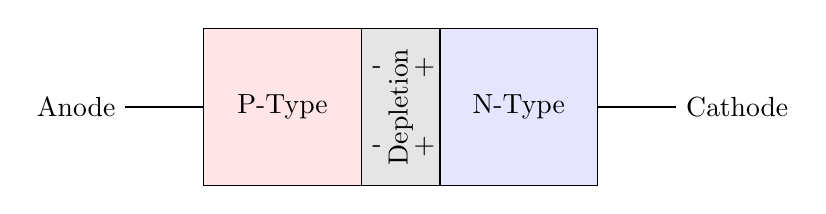
\begin{tikzpicture}
    % Block
    \draw[fill=red!10] (0,0) rectangle (2,2); \node at (1,1) {P-Type};
    \draw[fill=blue!10] (3,0) rectangle (5,2); \node at (4,1) {N-Type};
    
    % Depletion
    \draw[fill=gray!20] (2,0) rectangle (3,2); \node[rotate=90] at (2.5,1) {Depletion};
    
    % Terminals
    \draw (0,1) -- (-1,1) node[left] {Anode};
    \draw (5,1) -- (6,1) node[right] {Cathode};
    
    % Ions
    \node at (2.2, 1.5) {-}; \node at (2.2, 0.5) {-}; % Negative ions in P side? No, negative ions in P side near junction (Acceptor ions)
    \node at (2.8, 1.5) {+}; \node at (2.8, 0.5) {+}; % Positive ions in N side near junction (Donor ions)
    
\end{tikzpicture}
\captionof{figure}{PN Junction Structure}
\end{center}
\end{solutionbox}

\begin{mnemonicbox}
\mnemonic{BIRD: "Barrier forms at Interface, Rectifies Direct current"}
\end{mnemonicbox}

\questionmarks{3(a OR)}{3}{Explain working of photo diode.}

\begin{solutionbox}
\textbf{Answer}:

\textbf{Working of Photo Diode}:

\begin{itemize}
    \item \keyword{Operation}: Always operated in reverse bias
    \item \keyword{Dark Current}: Small leakage current flows when no light incident (due to thermal generation)
    \item \keyword{Light Incidence}: When light falls on junction, energy breaks covalent bonds
    \item \keyword{Carrier Generation}: Electron-hole pairs generated in depletion region
    \item \keyword{Photocurrent}: Electric field sweeps carriers across junction, increasing reverse current
    \item \keyword{Proportionality}: Current increases linearly with light intensity
\end{itemize}

\textbf{Diagram}:

\begin{center}
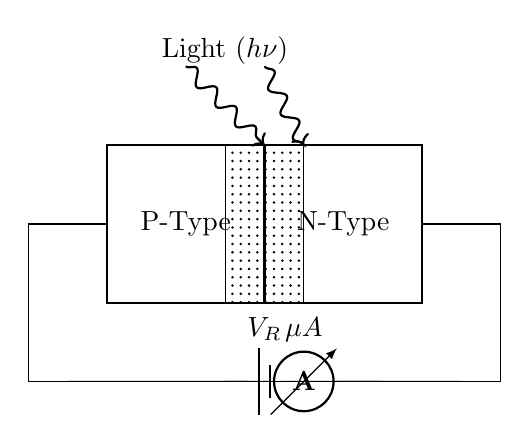
\begin{tikzpicture}
    \draw[thick] (0,0) rectangle (4,2);
    
    \draw[thick] (2,0) -- (2,2);
    \node at (1,1) {P-Type};
    \node at (3,1) {N-Type};
    \draw[pattern=dots] (1.5,0) rectangle (2.5,2);
    
    % Light
    \draw[->, thick, decorate, decoration={snake}] (1, 3) -- (2, 2);
    \draw[->, thick, decorate, decoration={snake}] (2, 3) -- (2.5, 2);
    \node at (1.5, 3.2) {Light ($h\nu$)};
    
    % Bias
    \draw (0,1) -- (-1,1) -- (-1, -1) -- (5, -1) -- (5, 1) -- (4,1);
    \draw (-0.5, -1) to[battery1, l=$V_R$] (4.5, -1); % Reverse Bias
    \draw (1.5, -1) to[ammeter, l=$\mu A$] (3.5, -1);
\end{tikzpicture}
\captionof{figure}{Photo Diode Operation}
\end{center}
\end{solutionbox}

\begin{mnemonicbox}
\mnemonic{DARK: "Dark current exists, Absorbs photons, Reverse bias, K-urrent increases"}
\end{mnemonicbox}

\questionmarks{3(b OR)}{4}{Explain P type semiconductor.}

\begin{solutionbox}
\textbf{Answer}:

\textbf{P-type Semiconductor}:

\textbf{Formation}:

\begin{itemize}
    \item \keyword{Base Material}: Intrinsic semiconductor (Si or Ge)
    \item \keyword{Doping Element}: Trivalent impurity (Boron, Aluminum, Indium, Gallium)
    \item \keyword{Process}: Adding trivalent atoms creates vacancies (holes)
\end{itemize}

\textbf{Characteristics}:

\begin{itemize}
    \item \keyword{Majority Carriers}: Holes (positive charge carriers)
    \item \keyword{Minority Carriers}: Electrons
    \item \keyword{Fermi Level}: Closer to valence band
    \item \keyword{Acceptor Ions}: Negative ions created when holes accept electrons
\end{itemize}

\textbf{Diagram}:

\begin{center}
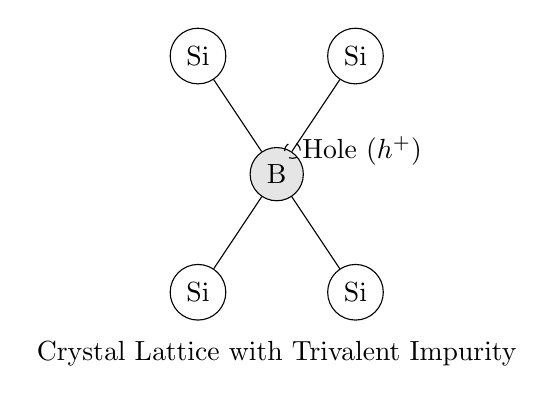
\begin{tikzpicture}
    \node[draw, circle] (Si1) at (0,0) {Si};
    \node[draw, circle] (Si2) at (2,0) {Si};
    \node[draw, circle, fill=gray!20] (B) at (1,1.5) {B};
    \node[draw, circle] (Si3) at (0,3) {Si};
    \node[draw, circle] (Si4) at (2,3) {Si};
    
    \draw (Si1) -- (B); \draw (Si2) -- (B); \draw (Si3) -- (B); \draw (Si4) -- (B);
    
    \node[circle, draw, dashed, inner sep=2pt] (h) at (1.2, 1.8) {};
    \node[right] at (h) {Hole ($h^+$)};
    
    \node[below] at (1, -0.5) {Crystal Lattice with Trivalent Impurity};
\end{tikzpicture}
\captionof{figure}{P-Type Doping}
\end{center}
\end{solutionbox}

\begin{mnemonicbox}
\mnemonic{TRIP: "Trivalent Impurity produces Positive holes"}
\end{mnemonicbox}

\questionmarks{3(c OR)}{7}{Compare half wave and full wave rectifier.}

\begin{solutionbox}
\textbf{Answer}:

\textbf{Comparison of Rectifiers}:

\begin{center}
\captionof{table}{Rectifier Comparison}
\begin{tabulary}{\linewidth}{|L|L|L|L|}
\hline
\textbf{Parameter} & \textbf{Half Wave} & \textbf{Full Wave (Center Tap)} & \textbf{Bridge Rectifier} \\ \hline
No. of Diodes & 1 & 2 & 4 \\ \hline
Max Efficiency & 40.6\% & 81.2\% & 81.2\% \\ \hline
Ripple Factor & 1.21 & 0.48 & 0.48 \\ \hline
Ripple Freq & $f_{in}$ & $2 f_{in}$ & $2 f_{in}$ \\ \hline
PIV Rating & $V_m$ & $2 V_m$ & $V_m$ \\ \hline
TUF & 0.287 & 0.693 & 0.812 \\ \hline
Output Voltage & $V_{dc} = V_m/\pi$ & $V_{dc} = 2V_m/\pi$ & $V_{dc} = 2V_m/\pi$ \\ \hline
Transformer & Simple & Center Tapped Required & Simple \\ \hline
Cost & Lowest & Medium & Highest (due to 4 diodes) \\ \hline
\end{tabulary}
\end{center}
\end{solutionbox}

\questionmarks{4(a)}{3}{Draw the symbol and construction of PNP and NPN transistor with proper labelling.}

\begin{solutionbox}
\textbf{Answer}:

\textbf{Construction and Symbols}:

\begin{center}
\begin{tikzpicture}
    % NPN Symbol
    \draw (0,2) node[npn, l=NPN] (Q1) {};
    \node[below] at (0, 1) {NPN Symbol};
    
    % PNP Symbol
    \draw (4,2) node[pnp, l=PNP] (Q2) {};
    \node[below] at (4, 1) {PNP Symbol};
    
    % NPN Construction
    \draw (0,-1) rectangle (3,-3);
    \draw (1,-1) -- (1,-3);
    \draw (2,-1) -- (2,-3);
    \node at (0.5,-2) {Emitter (N)};
    \node at (1.5,-2) {Base (P)};
    \node at (2.5,-2) {Collector (N)};
    \node[below] at (1.5, -3) {NPN Structure};
    
    % PNP Construction
    \draw (4,-1) rectangle (7,-3);
    \draw (5,-1) -- (5,-3);
    \draw (6,-1) -- (6,-3);
    \node at (4.5,-2) {Emitter (P)};
    \node at (5.5,-2) {Base (N)};
    \node at (6.5,-2) {Collector (P)};
    \node[below] at (5.5, -3) {PNP Structure};
\end{tikzpicture}
\captionof{figure}{Transistor Symbols and Construction}
\end{center}
\end{solutionbox}

\begin{mnemonicbox}
\mnemonic{P-POINT: "PNP Points In, NPN Points Out"}
\end{mnemonicbox}

\questionmarks{4(b)}{4}{Explain working of transistor amplifier.}

\begin{solutionbox}
\textbf{Answer}:

\textbf{Transistor Amplifier Working}:

\begin{itemize}
    \item \keyword{Biasing}: Emitter-Base junction is forward biased, Collector-Base junction is reverse biased (Active Region)
    \item \keyword{Input}: Weak AC signal applied across Emitter-Base
    \item \keyword{Control}: Small variations in Base current ($I_B$) cause large variations in Collector current ($I_C$)
    \item \keyword{Gain}: Current Gain $\beta = \Delta I_C / \Delta I_B$ is typically large (50-300)
    \item \keyword{Output}: Amplified voltage developed across load resistor connected in collector circuit
    \item \keyword{Process}: $I_E$ electrons injected into Base, most cross to Collector (due to reverse bias attraction), forming $I_C$
\end{itemize}

\textbf{Diagram}:

\begin{center}
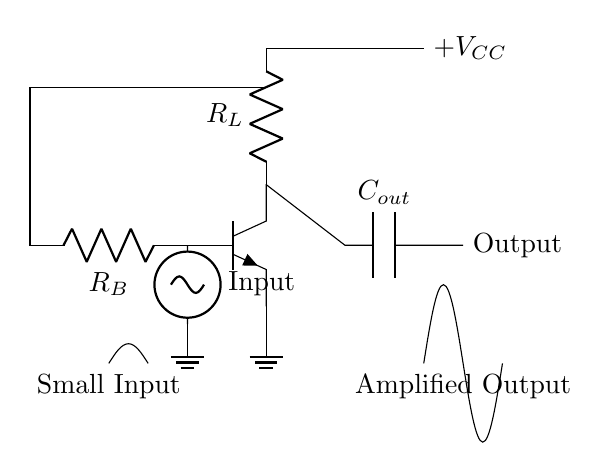
\begin{tikzpicture}
    \draw (0,0) node[npn] (Q) {};
    \draw (Q.E) -- (0,-1) node[ground] {};
    
    \draw (Q.B) -- (-1,0); 
    \draw (-1,0) to[sV, l=Input] (-1, -1) node[ground] {};
    \draw (-1, 0) to[R, l=$R_B$] (-3, 0) -- (-3, 2) -- (0, 2); % Bias? Simplified.
    
    \draw (Q.C) to[R, l=$R_L$] (0, 2.5);
    \draw (0, 2.5) -- (2, 2.5) node[right] {$+V_{CC}$};
    
    \draw (Q.C) -- (1, 0) to[C, l=$C_{out}$] (2,0) -- (2.5,0) node[right] {Output};
    
    % Waveforms
    \draw (-2, -1.5) sin (-1.75, -1.25) cos (-1.5, -1.5);
    \node at (-2, -1.8) {Small Input};
    
    \draw (2, -1.5) sin (2.25, -0.5) cos (2.5, -1.5) sin (2.75, -2.5) cos (3, -1.5);
    \node at (2.5, -1.8) {Amplified Output};
\end{tikzpicture}
\captionof{figure}{Common Emitter Amplifier Concept}
\end{center}
\end{solutionbox}

\questionmarks{4(c)}{7}{Explain working of Zener diode.}

\begin{solutionbox}
\textbf{Answer}:

\textbf{Zener Diode}:

\textbf{Construction}:
\begin{itemize}
    \item Heavily doped P-N junction diode
    \item Designed to operate in reverse breakdown region
\end{itemize}

\textbf{Working Principle}:
\begin{itemize}
    \item \keyword{Forward Bias}: Acts like normal diode
    \item \keyword{Reverse Bias}: Blocks current up to breakdown voltage ($V_Z$)
    \item \keyword{Breakdown}: At $V_Z$, sharp increase in current occurs due to Zener effect (quantum tunneling) or Avalanche effect
    \item \keyword{Voltage Regulation}: Voltage across diode remains constant ($V_Z$) despite large changes in current
\end{itemize}

\textbf{Applications}:
\begin{itemize}
    \item Voltage Regulator
    \item Reference voltage source
    \item Over-voltage protection
\end{itemize}

\textbf{Characteristics Diagram}:

\begin{center}
\begin{tikzpicture}
    \draw[->] (-3,0) -- (3,0) node[right] {$V$};
    \draw[->] (0,-3) -- (0,3) node[above] {$I$};
    
    % Forward
    \draw[thick, blue] (0,0) -- (0.7,0) .. controls (0.8,0.1) and (0.9,1) .. (1,2.5);
    \node at (1.5, 1) {Forward};
    
    % Reverse
    \draw[thick, blue] (0,0) -- (-2,0) -- (-2,-2.5);
    \node[below] at (-2,0) {$V_Z$};
    \node[left] at (-2, -1) {Breakdown};
    \node[left] at (-0.5, -2) {Reverse};
\end{tikzpicture}
\captionof{figure}{Zener V-I Characteristics}
\end{center}
\end{solutionbox}

\begin{mnemonicbox}
\mnemonic{ZAP: "Zener Always Provides constant voltage"}
\end{mnemonicbox}

\questionmarks{4(a OR)}{3}{Explain transistor as a switch.}

\begin{solutionbox}
\textbf{Answer}:

\textbf{Transistor as Switch}:
Operates in Cut-off and Saturation regions.

\begin{itemize}
    \item \keyword{OFF State (Open Switch)}:
        \begin{itemize}
            \item Base current $I_B = 0$
            \item Operates in \textbf{Cut-off Region}
            \item Collector current $I_C \approx 0$
            \item Output voltage $V_{CE} = V_{CC}$
        \end{itemize}
    \item \keyword{ON State (Closed Switch)}:
        \begin{itemize}
            \item Sufficient Base current supplied
            \item Operates in \textbf{Saturation Region}
            \item Maximum Collector current flows ($I_{sat}$)
            \item Output voltage $V_{CE} \approx 0.2V$ (Saturation voltage)
        \end{itemize}
\end{itemize}

\textbf{Diagram}:

\begin{center}
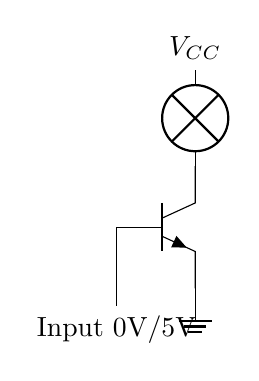
\begin{tikzpicture}
    \draw (0,0) node[npn] (Q) {};
    \draw (Q.E) node[ground] {};
    \draw (Q.C) to[lamp] (0, 2) node[above] {$V_{CC}$};
    \draw (Q.B) -- (-1,0); 
    \draw (-1, 0) -- (-1, -1) node[below] {Input 0V/5V};
\end{tikzpicture}
\captionof{figure}{Transistor Switch Circuit}
\end{center}
\end{solutionbox}

\begin{mnemonicbox}
\mnemonic{CO-SI: "Cut-off is Open, Saturation is Closed"}
\end{mnemonicbox}

\questionmarks{4(b OR)}{4}{Draw and explain characteristics of CE amplifier.}

\begin{solutionbox}
\textbf{Answer}:

\textbf{Common Emitter Characteristics}:

\textbf{1. Input Characteristics} ($I_B$ vs $V_{BE}$ at constant $V_{CE}$):
\begin{itemize}
    \item Resembles forward biased diode characteristic
    \item Beyond knee voltage (0.7V for Si), $I_B$ increases rapidly with small increase in $V_{BE}$
    \item Increasing $V_{CE}$ shifts curve slightly to right (Early effect - ignoring for basic explanation)
\end{itemize}

\textbf{2. Output Characteristics} ($I_C$ vs $V_{CE}$ at constant $I_B$):
\begin{itemize}
    \item \keyword{Cut-off Region}: $I_B=0$, $I_C \approx 0$. Transistor OFF.
    \item \keyword{Active Region}: $I_C$ is constant for given $I_B$, almost independent of $V_{CE}$. Used for amplification. Linear region.
    \item \keyword{Saturation Region}: $V_{CE}$ is very low ($<0.2V$). $I_C$ increases rapidly with $V_{CE}$. Transistor ON.
\end{itemize}

\textbf{Diagram}:

\begin{center}
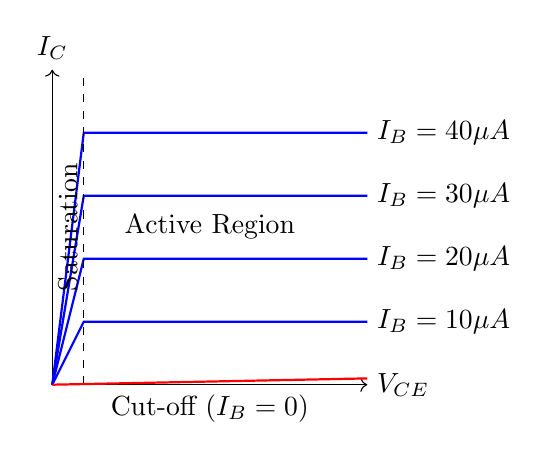
\begin{tikzpicture}[scale=0.8]
    % Output Char
    \draw[->] (0,0) -- (5,0) node[right] {$V_{CE}$};
    \draw[->] (0,0) -- (0,5) node[above] {$I_C$};
    
    \foreach \y/\Ib in {1/10, 2/20, 3/30, 4/40} {
        \draw[thick, blue] (0,0) -- (0.5, \y) -- (5, \y);
        \node[right] at (5, \y) {$I_B=\Ib\mu A$};
    }
    
    \draw[dashed] (0.5, 0) -- (0.5, 5);
    \node[rotate=90] at (0.25, 2.5) {Saturation};
    
    \node at (2.5, 2.5) {Active Region};
    
    \draw[thick, red] (0,0) -- (5,0.1);
    \node[below] at (2.5, 0) {Cut-off ($I_B=0$)};
\end{tikzpicture}
\captionof{figure}{CE Output Characteristics}
\end{center}
\end{solutionbox}

\questionmarks{4(c OR)}{7}{Explain working of varactor diode.}

\begin{solutionbox}
\textbf{Answer}:

\textbf{Working of Varactor Diode}:

\begin{itemize}
    \item \keyword{Function}: Acts as a voltage-controlled variable capacitor
    \item \keyword{Operation}: Always operated in reverse bias
    \item \keyword{Principle}: 
        \begin{itemize}
            \item Reverse bias voltage increases width of depletion region
            \item Depletion region acts as dielectric between P and N regions (acting as plates)
            \item Capacitance $C = \epsilon A / d$ (where $d$ is depletion width)
            \item As Reverse Voltage ($V_R$) increases $\rightarrow$ Width ($d$) increases $\rightarrow$ Capacitance ($C$) decreases
        \end{itemize}
    \item \keyword{Relationship}: $C_T \propto \frac{1}{\sqrt{V_R}}$
    \item \keyword{Application}: Tuning circuits (Radio/TV tuners), VCOs (Voltage Controlled Oscillators)
\end{itemize}

\textbf{Diagram}:

\begin{center}
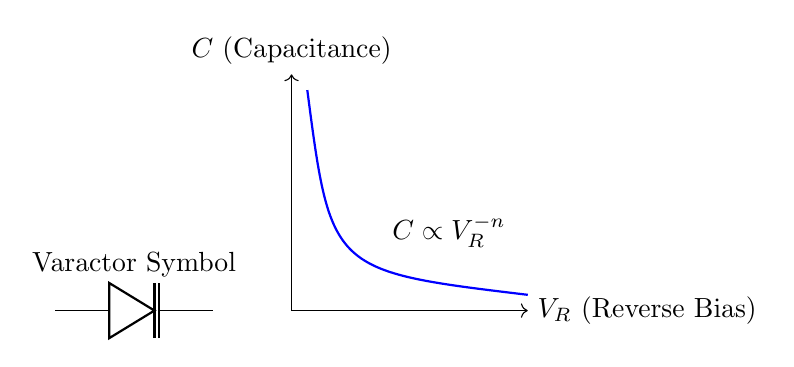
\begin{tikzpicture}
    % Symbol
    \draw (0,0) to[varcap, l=Varactor Symbol] (2,0);
    
    % Graph
    \draw[->] (3,0) -- (6,0) node[right] {$V_R$ (Reverse Bias)};
    \draw[->] (3,0) -- (3,3) node[above] {$C$ (Capacitance)};
    \draw[thick, blue] (3.2, 2.8) .. controls (3.5, 0.5) .. (6, 0.2);
    \node at (5, 1) {$C \propto V_R^{-n}$};
\end{tikzpicture}
\captionof{figure}{Varactor Diode Characteristics}
\end{center}
\end{solutionbox}

\begin{mnemonicbox}
\mnemonic{VARY: "Voltage Adjusts Reverse-bias Yielding capacitance"}
\end{mnemonicbox}

\questionmarks{5(a)}{3}{Define Active, Saturation and Cut-Off region for transistor amplifier.}

\begin{solutionbox}
\textbf{Answer}:

\begin{itemize}
    \item \keyword{Active Region}: 
        \begin{itemize}
            \item Emitter-Base junction: Forward Biased
            \item Collector-Base junction: Reverse Biased
            \item Use: Amplification
        \end{itemize}
    \item \keyword{Saturation Region}:
        \begin{itemize}
            \item Emitter-Base junction: Forward Biased
            \item Collector-Base junction: Forward Biased
            \item Use: ON Switch (Closed)
        \end{itemize}
    \item \keyword{Cut-Off Region}:
        \begin{itemize}
            \item Emitter-Base junction: Reverse Biased
            \item Collector-Base junction: Reverse Biased
            \item Use: OFF Switch (Open)
        \end{itemize}
\end{itemize}
\end{solutionbox}

\questionmarks{5(b)}{4}{Check current gain $\alpha$ and $\beta$ if $I_c = 10mA$ and $I_b = 100\mu A$.}

\begin{solutionbox}
\textbf{Answer}:

\textbf{Given}:
\begin{itemize}
    \item $I_C = 10 mA$
    \item $I_B = 100 \mu A = 0.1 mA$
\end{itemize}

\textbf{Calculations}:

1. \textbf{Calculate $\beta$}:
   \[ \beta = \frac{I_C}{I_B} = \frac{10 mA}{0.1 mA} = 100 \]

2. \textbf{Calculate Emitter Current $I_E$}:
   \[ I_E = I_C + I_B = 10 mA + 0.1 mA = 10.1 mA \]

3. \textbf{Calculate $\alpha$}:
   \[ \alpha = \frac{I_C}{I_E} = \frac{10 mA}{10.1 mA} \approx 0.9901 \]
   
   \textit{Alternatively using relation}:
   \[ \alpha = \frac{\beta}{1+\beta} = \frac{100}{101} \approx 0.9901 \]

\textbf{Result}:
\begin{itemize}
    \item $\beta = 100$
    \item $\alpha = 0.99$
\end{itemize}
\end{solutionbox}

\questionmarks{5(c)}{7}{Discuss strategies for Electronic Waste management in small electronic industries.}

\begin{solutionbox}
\textbf{Answer}:

\textbf{E-Waste Management Strategies}:

\begin{enumerate}
    \item \keyword{Inventory Management}: Keep track of all electronic equipment and lifespan to plan replacements efficiently.
    \item \keyword{Reduce}: Minimize purchase of unnecessary equipment. Opt for upgradable modular devices instead of replacing entire units.
    \item \keyword{Reuse}: refurbish old electronics for less demanding tasks (e.g., using older PCs for data entry or print servers).
    \item \keyword{Recycle}: Partner with certified e-waste recyclers who safely extract valuable metals (Au, Ag, Cu) and dispose of hazardous materials (Pb, Hg).
    \item \keyword{Segregation}: Set up separate bins for e-waste (batteries, cables, circuit boards) to prevent mixing with general waste.
    \item \keyword{EPR Compliance}: Adhere to Extended Producer Responsibility (EPR) guidelines if involved in manufacturing.
    \item \keyword{Employee Training}: Educate staff about proper disposal methods and data wiping before disposal.
\end{enumerate}

\textbf{Diagram}:

\begin{center}
\begin{tikzpicture}[node distance=2cm]
    \node [gtu block] (Gen) {Generation};
    \node [gtu block, right=of Gen] (Col) {Collection};
    \node [gtu block, right=of Col] (Seg) {Segregation};
    \node [gtu block, below=of Seg] (Rec) {Recycling};
    \node [gtu block, left=of Rec] (Ref) {Refurbish/Reuse};
    \node [gtu block, left=of Ref] (Dis) {Disposal (Last Resort)};

    \path [gtu arrow] (Gen) -- (Col);
    \path [gtu arrow] (Col) -- (Seg);
    \path [gtu arrow] (Seg) -- (Rec);
    \path [gtu arrow] (Seg) -- (Ref);
    \path [gtu arrow] (Rec) -- (Dis);
\end{tikzpicture}
\captionof{figure}{E-Waste Flow}
\end{center}
\end{solutionbox}

\begin{mnemonicbox}
\mnemonic{3R: "Reduce, Reuse, Recycle"}
\end{mnemonicbox}

\questionmarks{5(a OR)}{3}{Draw circuit configuration of CB, CE and CC transistor.}

\begin{solutionbox}
\textbf{Answer}:

\begin{center}
\begin{tikzpicture}[scale=0.8]
    % CB
    \draw (0,0) node[npn, l=CB, rotate=270] (Q1) {};
    \node[below] at (0,-1) {Common Base};
    % Base Grounded
    \draw (Q1.B) node[ground] {};
    
    % CE
    \draw (4,0) node[npn, l=CE] (Q2) {};
    \node[below] at (4,-1) {Common Emitter};
    % Emitter Grounded
    \draw (Q2.E) node[ground] {};
    
    % CC
    \draw (8,0) node[npn, l=CC] (Q3) {};
    \node[below] at (8,-1) {Common Collector};
    % Collector Grounded (AC ground usually VCC)
    \draw (Q3.C) node[ground] {}; 
    % Note: Strictly CC connects C to VCC, which is AC ground. Symbolically this is acceptable for config diagram.
    
\end{tikzpicture}
\captionof{figure}{Transistor Configurations}
\end{center}
\end{solutionbox}

\questionmarks{5(b OR)}{4}{Derive the relation between current gain $\alpha$ and $\beta$.}

\begin{solutionbox}
\textbf{Answer}:

\textbf{Derivation}:

1. We know transistor currents:
   \[ I_E = I_C + I_B \]

2. Divide entire equation by $I_C$:
   \[ \frac{I_E}{I_C} = \frac{I_C}{I_C} + \frac{I_B}{I_C} \]
   \[ \frac{1}{\alpha} = 1 + \frac{1}{\beta} \]
   (Because $\alpha = I_C/I_E$ and $\beta = I_C/I_B$)

3. Solve for $\alpha$:
   \[ \frac{1}{\alpha} = \frac{\beta + 1}{\beta} \]
   \[ \alpha = \frac{\beta}{1+\beta} \]

4. Solve for $\beta$:
   \[ \frac{1}{\beta} = \frac{1}{\alpha} - 1 = \frac{1 - \alpha}{\alpha} \]
   \[ \beta = \frac{\alpha}{1-\alpha} \]

\textbf{Conclusion}:
\[ \alpha = \frac{\beta}{1+\beta}, \quad \beta = \frac{\alpha}{1-\alpha} \]
\end{solutionbox}

\questionmarks{5(c OR)}{7}{Define E-waste and explain disposal of Electronic waste.}

\begin{solutionbox}
\textbf{Answer}:

\textbf{Definition}:
\keyword{E-Waste (Electronic Waste)} refers to discarded electrical or electronic devices such as computers, phones, printers, and appliances that have reached the end of their useful life.

\textbf{Disposal Methods}:

\begin{enumerate}
    \item \keyword{Landfilling}: Dumping waste in trenches. Least preferred method as toxic substances (Lead, Cadmium) leach into soil and groundwater.
    \item \keyword{Incineration}: Controlled burning of waste. reduces volume but can release toxic gases into atmosphere if not filtered properly.
    \item \keyword{Acid Bath}: Soaking circuits in acid to extract gold. Highly hazardous to workers and environment.
    \item \keyword{Mechanical Recycling (Preferred)}:
        \begin{itemize}
            \item Shredding: Breaking devices into small pieces.
            \item Separation: Using magnets and eddy currents to separate metals from plastic.
            \item Recovery: Smelting metals for reuse.
        \end{itemize}
    \item \keyword{Reuse/Refurbishing}: Extending life by repairing. Best for environment.
\end{enumerate}

\textbf{Pyramid of E-Waste}:

\begin{center}
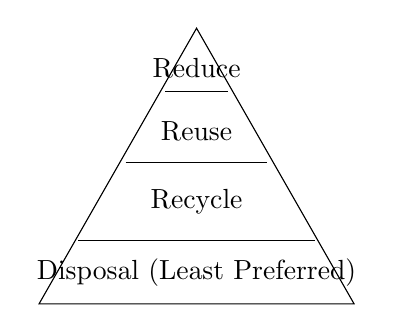
\begin{tikzpicture}
    \draw (0,0) -- (4,0) -- (2,3.5) -- cycle;
    \draw (0.5, 0.8) -- (3.5, 0.8);
    \draw (1.1, 1.8) -- (2.9, 1.8);
    \draw (1.6, 2.7) -- (2.4, 2.7);
    
    \node at (2, 0.4) {Disposal (Least Preferred)};
    \node at (2, 1.3) {Recycle};
    \node at (2, 2.2) {Reuse};
    \node at (2, 3) {Reduce};
\end{tikzpicture}
\captionof{figure}{Waste Management Hierarchy}
\end{center}
\end{solutionbox}

\end{document}

